\section{Related Work}\label{relatedWork}
%Camera Path Animator 3.0 (Unity asset store).
%Camera system that follows the character but also focuses on showing the environment - Used in the game God of War.

\begin{figure*}[htbp]
\centering
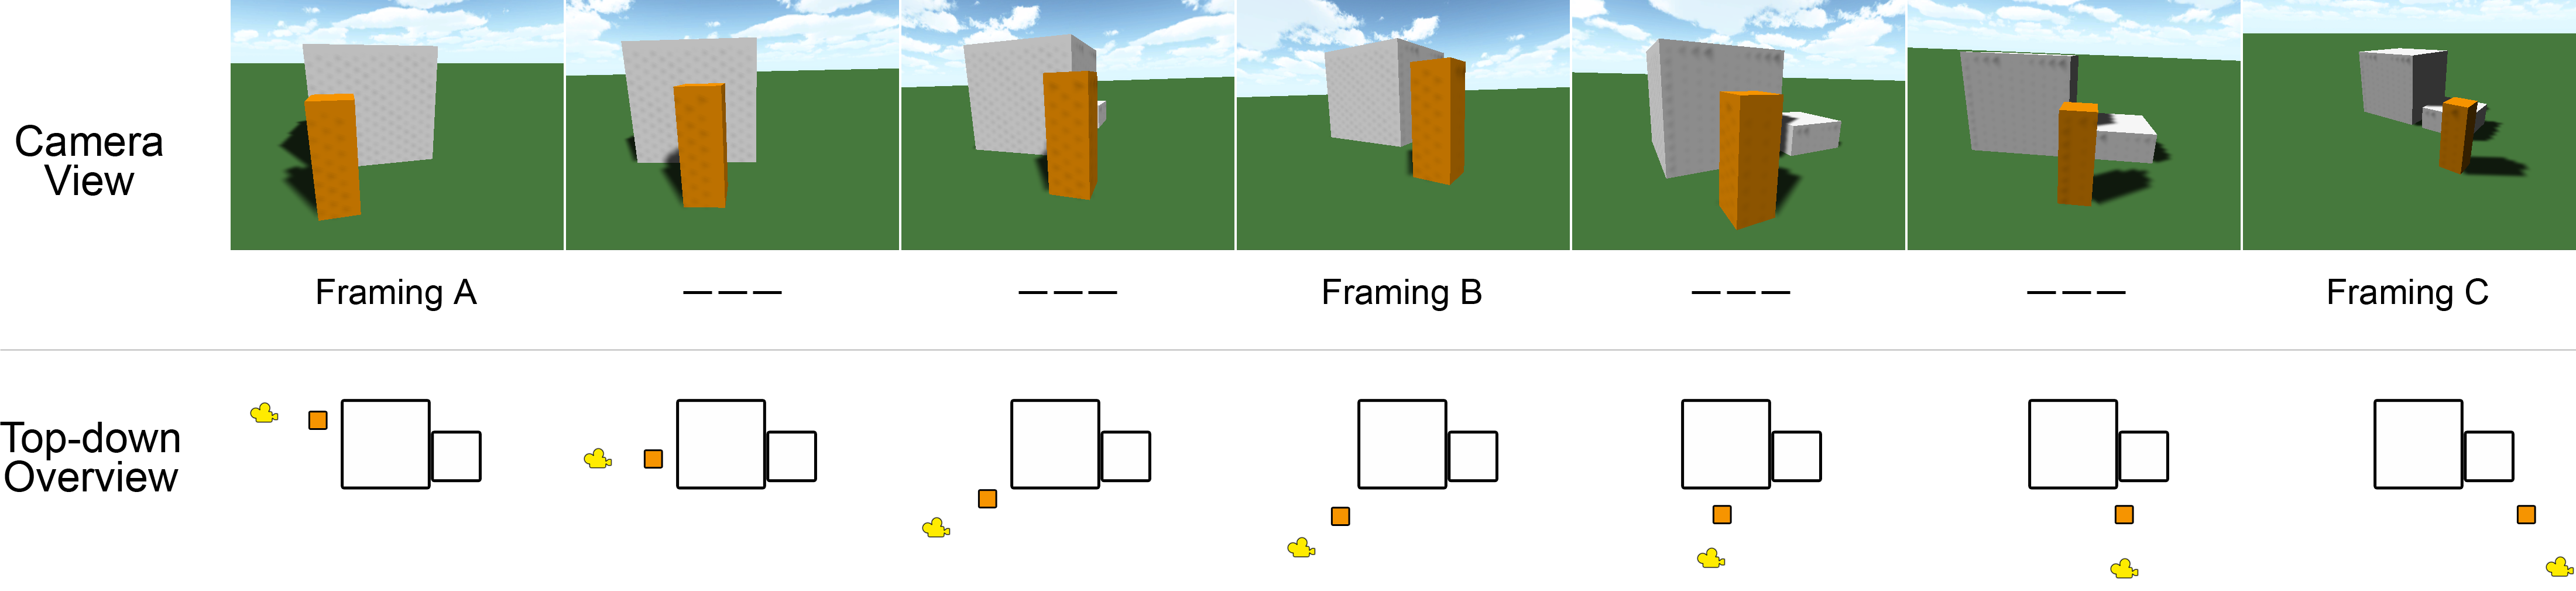
\includegraphics[width=1\textwidth]{Pics/InterpolationExample}
\caption{An example of a camera interpolation between three framings (A, B and C). The framings contain position, rotation and field of view. As the player character (orange cube) moves, the camera follows him by interpolating between the framings.}
\label{fig:InterpolationExample}
\end{figure*}

Automatic camera control is an active research field. In 3D computer animation, a virtual environment is rendered in frames from a specific point of view. This is a complex process that involves technical and artistic tasks, typically requiring the work of several professionals for a long time period \cite{burelli_automatic_2014}. Developing a system that makes the camera animation automatic can be beneficial at both a professional level (to reduce cost) or at an amateur level (to increase quality). Systems that emphasize automatic behaviour have been proposed \cite{bourne_constraintBased_2008, burelli_automatic_2014}; these use an automatic approach for controlling a virtual camera driven by AI techniques. However, the focus of the camera tool proposed in this work is on artistic control. Hence, an automatic approach is not feasible.

In a behind-the-scenes documentary, the developers behind the PlayStation game series \textit{God of War}, talk about the importance of being able to frame the scene \cite{gow_camera}. Depending on the context, it is important for them to frame the scene, so players know where they should be heading next. They use camera zones to determine what area the player is in and then activate the corresponding camera for that zone. This example shows that it is important that the artists are able to crate framings themselves.

The main requirement of a framing-based camera tool for games is that it can go from one camera setting (A) to another camera setting (B) depending on the player's position or certain events. For instance, A and B can be different in position, rotation and field of view.
%By looking at games with emphasis on its visuals and environments, it was found that the camera changes its position, rotation and field of view. 
Figure \ref{fig:InterpolationExample} shows an example of how the camera interpolates between three positions.

%\begin{figure}[htbp]
%\centering
%
\includegraphics[width=.4\textwidth]{Pics/CameraSystem_BASIC}
%\caption{The camera interpolates between position A and B. A and B contain information about its %position, rotation and field of view.}
%\label{fig:CameraSystem_BASIC}
%\end{figure}

%\subsection{Camera Tools}
The tool Camera Path Animator \cite{unity_camTool} can be used for creating animated cameras within the game engine Unity. As the name suggests, it works by animating the camera along a specified path, which can have various shapes (e.g., Bezier and Hermite curves). The tool is primarily targeted towards creating cameras that move linearly along a set path, i.e. for use in cinematic sequences. It provides various ways of inserting, moving and deleting points, as well as changing settings such as field of view, speed, interpolation type and easing. Additionally, it has an event system for triggering certain events at certain points in the path. For this project, it was important that the interface and the framings are created is customized for the artists; hence, we chose not to extend the Camera Path Animator, but instead took inspiration from it.

%Why we don't use Camera Path Animator:
%Customizable interface
%Specific for artists
%Freedom
%Flexibility
%Maya knowledge
%Path

%\begin{figure}[htbp]
%\centering
%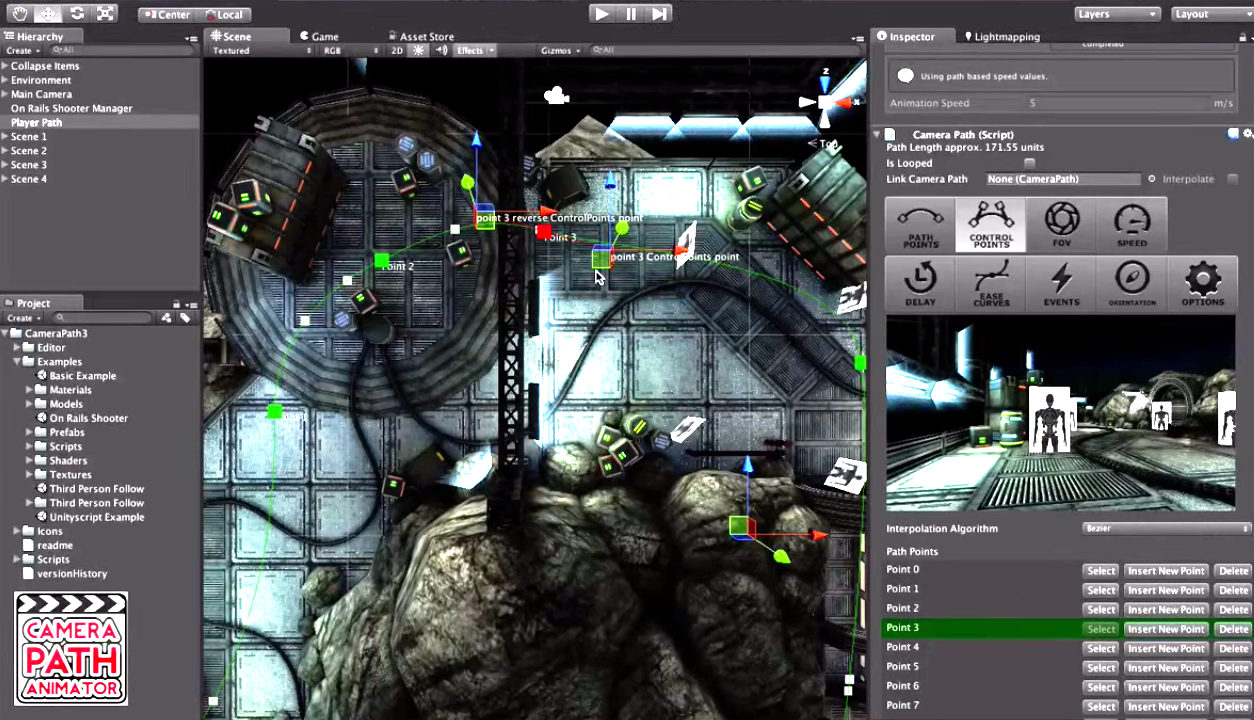
\includegraphics[width=0.40\textwidth]{Pics/unity_path_cam_tool}
%\caption{Overview of the objects related to the camera system.}
%\label{fig:unity_path_cam_tool}
%\end{figure}

%The God of War video game franchise for the PlayStation systems has also made notable use of their camera systems. The developers call the system Rail Driven Cameras and consists of a 'rail' that will be placed in the game world. A camera is keyed in both ends of the rail, and the camera will then animate between them as the protagonist moves along the rail. % Det her føles pølse, ikke meget at skrive om det og super unscientific

%\begin{figure}[htbp]
%\centering
%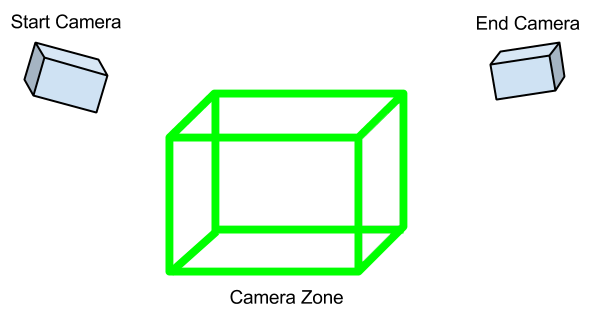
\includegraphics[width=0.45\textwidth]{Pics/gow_cameraZones2}
%\caption{When the player enters a camera zone, the camera will interpolate between the two pre-%defined cameras associated with that zone.}
%\lab%el{fig:gow_zones}
%\end{figure}

%\begin{figure}[htbp]
%\centering
%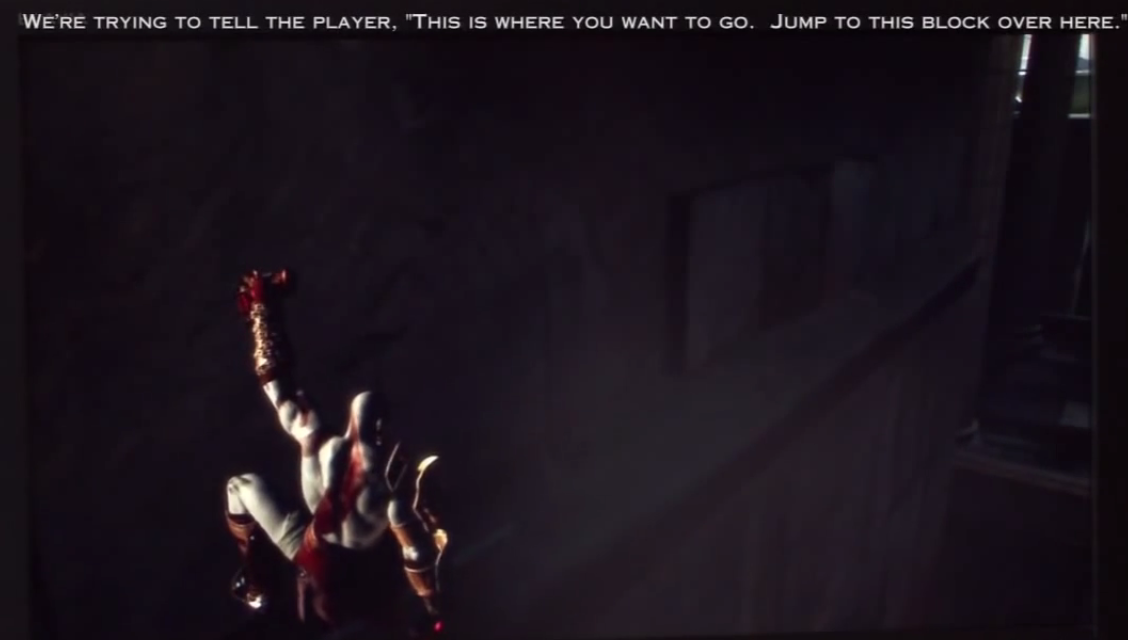
\includegraphics[width=0.40\textwidth]{Pics/gow_next}
%\caption{The camera's framing can help the designer guide the player in the right direction.}
%\label{fig:gow_jump}
%\end{figure}


%An example of this is when the main character has to jump from one 



%\textbf{Scientific material: Write about automatic camera tools (Paulo something-something) - even though we are not using it. Make it clear that our work is different from how other people's camera tools work}

%\subsection{Participatory Design}
Participatory design has been defined as the participation of users in the design process of a system that is to be implemented in an organization \cite{kensing_participatory_1998}. By involving users in the design, their skills, experiences, and interests are taken into consideration, thereby increasing the likelihood that the system will be useful to them.

According to participatory design researchers, it is important that there is an active cooperation between the designer and the user \cite{kensing_participatory_1998}. This results in the designer gaining knowledge of the user's current work practices, and the user gaining knowledge of the technology being developed. It is also important that users take an active part in the analysis of needs, selection of technology, design and prototyping, as well as organizational implementation.